\chapter{Thực thi, đo lường và đánh giá}

\reportsection{I. Giao tiếp 2 chiều}

Trong giai đoạn giao tiếp 2 chiều, hệ thống được vận hành với hai nút ESP32 tham gia
cùng một bus CAN để kiểm tra khả năng gửi và nhận bản tin theo cả hai chiều. Mục tiêu
của phần này là chứng minh rằng mô hình phần cứng và firmware hiện tại có thể duy trì
trao đổi dữ liệu ổn định trước khi đưa thêm các kịch bản tấn công và cơ chế phòng thủ.

\IfFileExists{images/mach_2_node.png}{%
\begin{figure}[H]
  \centering
  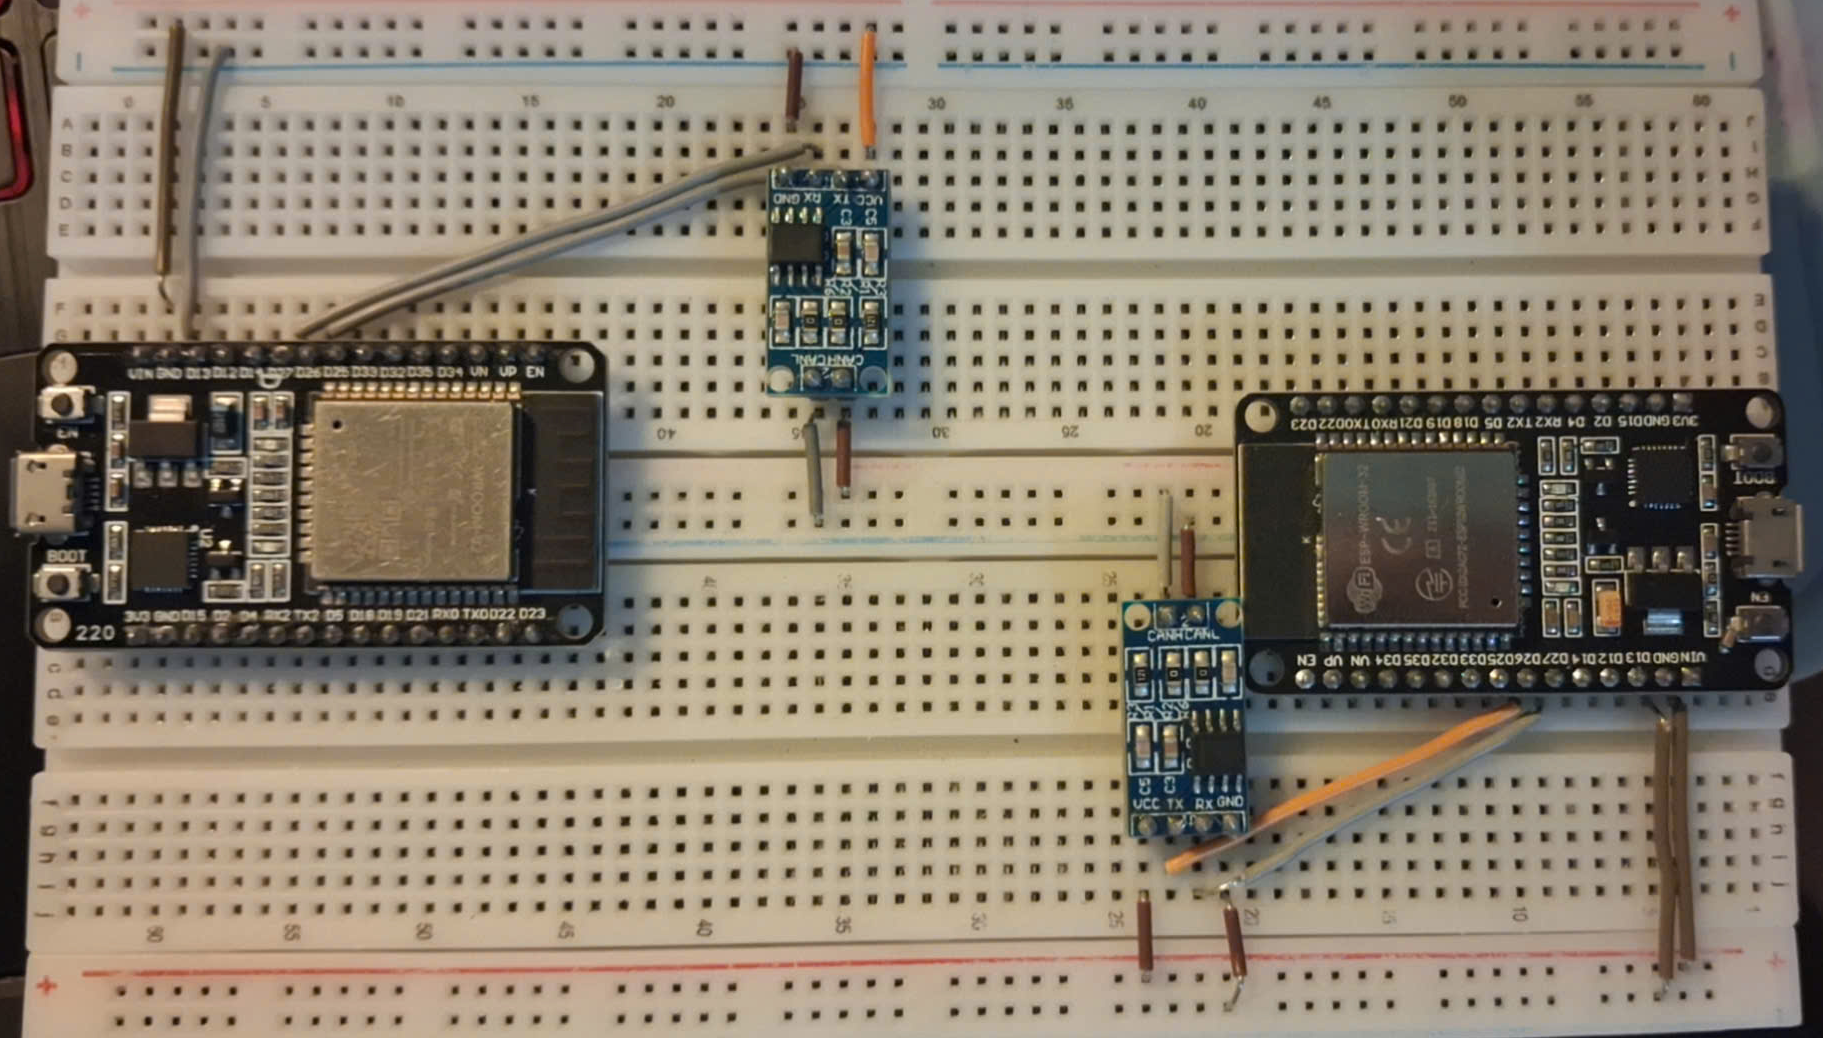
\includegraphics[width=0.62\textwidth]{images/mach_2_node.png}
  \caption{Mô hình phần cứng giao tiếp CAN với 2 node ESP32}
  \label{fig:mach-2-node}
\end{figure}
}{%
\placeholderfigure{Ảnh mạch thực tế khi hệ thống chỉ gồm 2 node ESP32 giao tiếp qua CAN}{Mô
hình phần cứng giao tiếp CAN với 2 node ESP32}
}

\IfFileExists{images/ch6-can-two-way-web.png}{%
\begin{figure}[H]
  \centering
  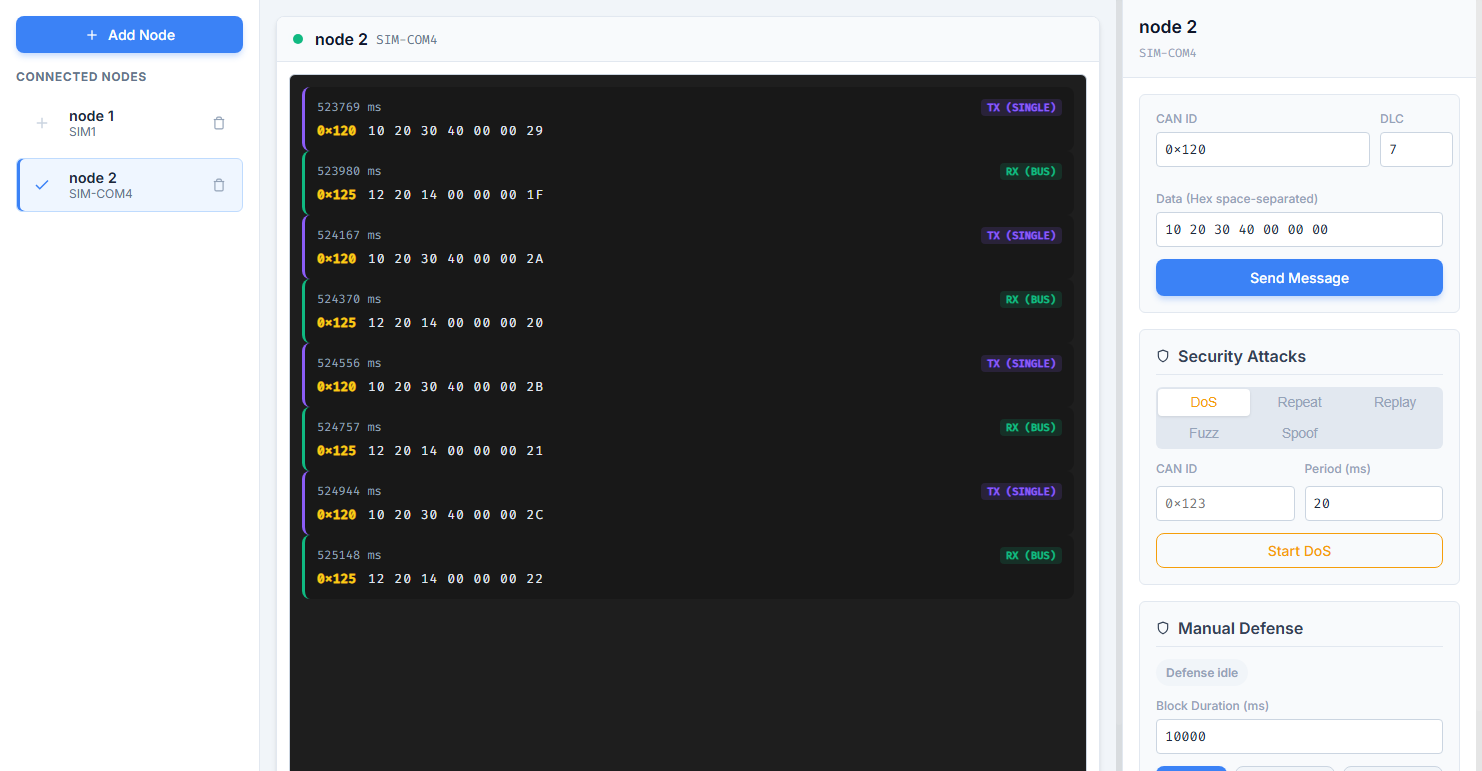
\includegraphics[width=0.98\textwidth]{images/ch6-can-two-way-web.png}
  \caption{Phiên giao tiếp CAN hai chiều bình thường hiển thị trên giao diện web}
  \label{fig:can-two-way-web}
\end{figure}
}

Ảnh chụp ở Hình \ref{fig:can-two-way-web} cho thấy nút \texttt{node 2} vừa phát khung CAN
ID \texttt{0x120} vừa nhận khung ID \texttt{0x125} từ nút còn lại trên cùng bus. Các bản tin TX
và RX xuất hiện xen kẽ, đồng thời byte cuối của dữ liệu thay đổi tuần tự theo từng lần gửi.

\reportsection{II. Các kịch bản tấn công và phản ứng phòng thủ}

Để mô phỏng tấn công trên mạng CAN, hệ thống bổ sung thêm một nút thứ ba đóng vai trò
thiết bị tấn công. Nút này có nhiệm vụ quan sát lưu lượng hợp lệ trên bus, lưu lại bản tin đã
thu được và phát lại hoặc phát dồn với chu kỳ xác định nhằm kiểm tra khả năng chịu lỗi của
hệ thống truyền nhận.

\IfFileExists{images/mo-hinh-thuc-nghiem.png}{%
\begin{figure}[H]
  \centering
  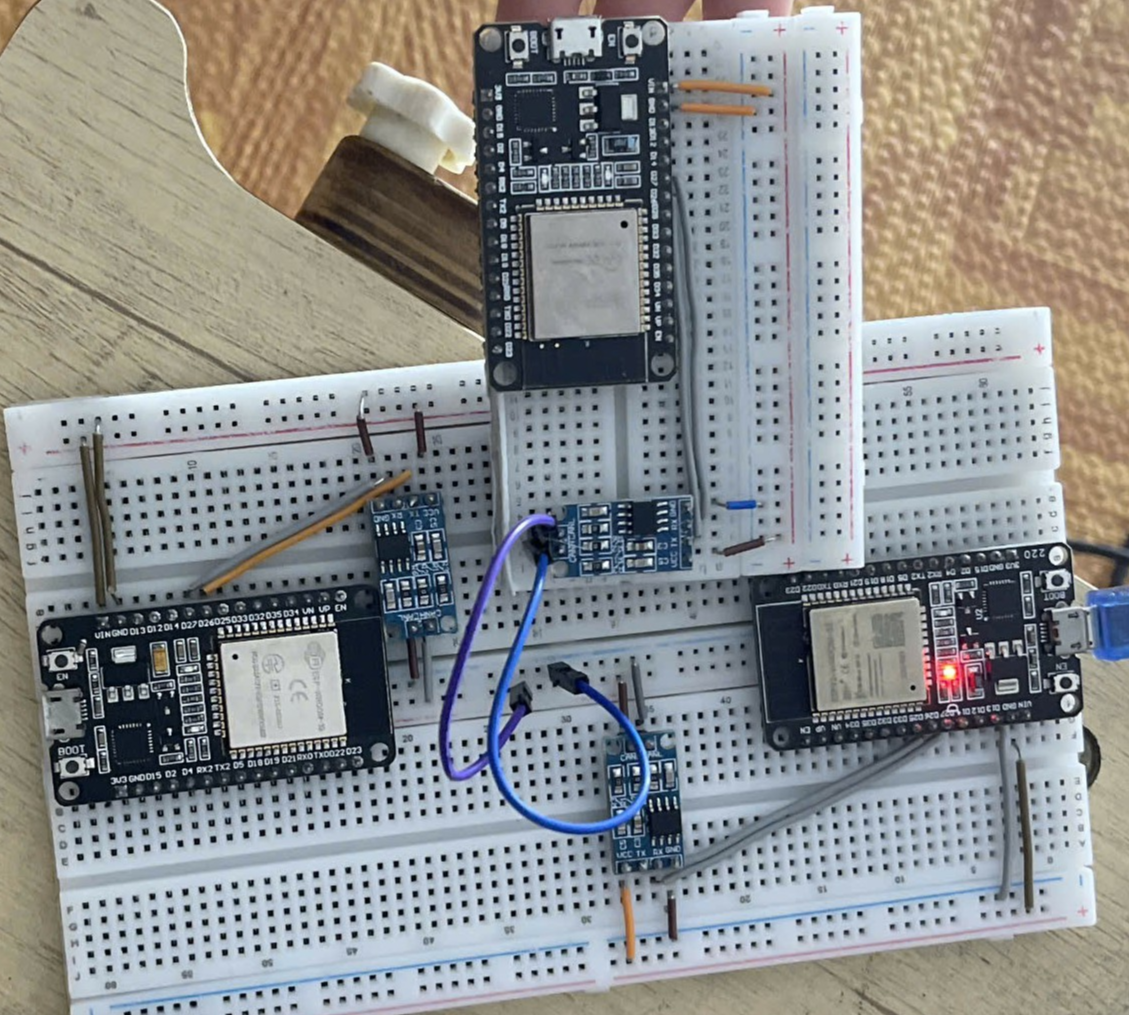
\includegraphics[width=0.72\textwidth]{images/mo-hinh-thuc-nghiem.png}
  \caption{Mô hình phần cứng thực tế khi bổ sung thêm node hacker vào bus CAN}
  \label{fig:mach-hacker}
\end{figure}
}{%
\placeholderfigure{Ảnh mô hình phần cứng khi bổ sung thêm nút tấn công vào bus CAN}{Mạch
giao tiếp CAN thêm phần tử Hacker}
}

Trên giao diện điều khiển, người vận hành có thể chọn nút đang thao tác, cấu hình tham số
tấn công và theo dõi phản hồi của từng nút theo thời gian thực. Để phần đánh giá rõ ràng
hơn, chương này trình bày theo từng kịch bản riêng gồm DoS, Replay, Fuzzing và Spoofing.
Trong mỗi kịch bản, kết quả được mô tả theo hai bước liên tiếp: bước hệ thống sinh cảnh báo
\texttt{ALERT} và bước người vận hành kích hoạt \texttt{defense} để chặn hoặc giảm tác động
của lưu lượng bất thường lên nút nhận.

\reportsubsection{1. Tấn công DoS}

Trong kịch bản DoS, nút tấn công phát liên tiếp nhiều khung CAN cùng một ID với chu kỳ rất
ngắn để làm tăng nhanh mật độ lưu lượng trên bus. Mục tiêu của phần này là kiểm tra khả
năng quan sát hiện tượng ngập bản tin ở nút nhận và khả năng sinh cảnh báo khi tốc độ khung
vượt ngưỡng bình thường.

\IfFileExists{images/dos_alert.png}{%
\begin{figure}[H]
  \centering
  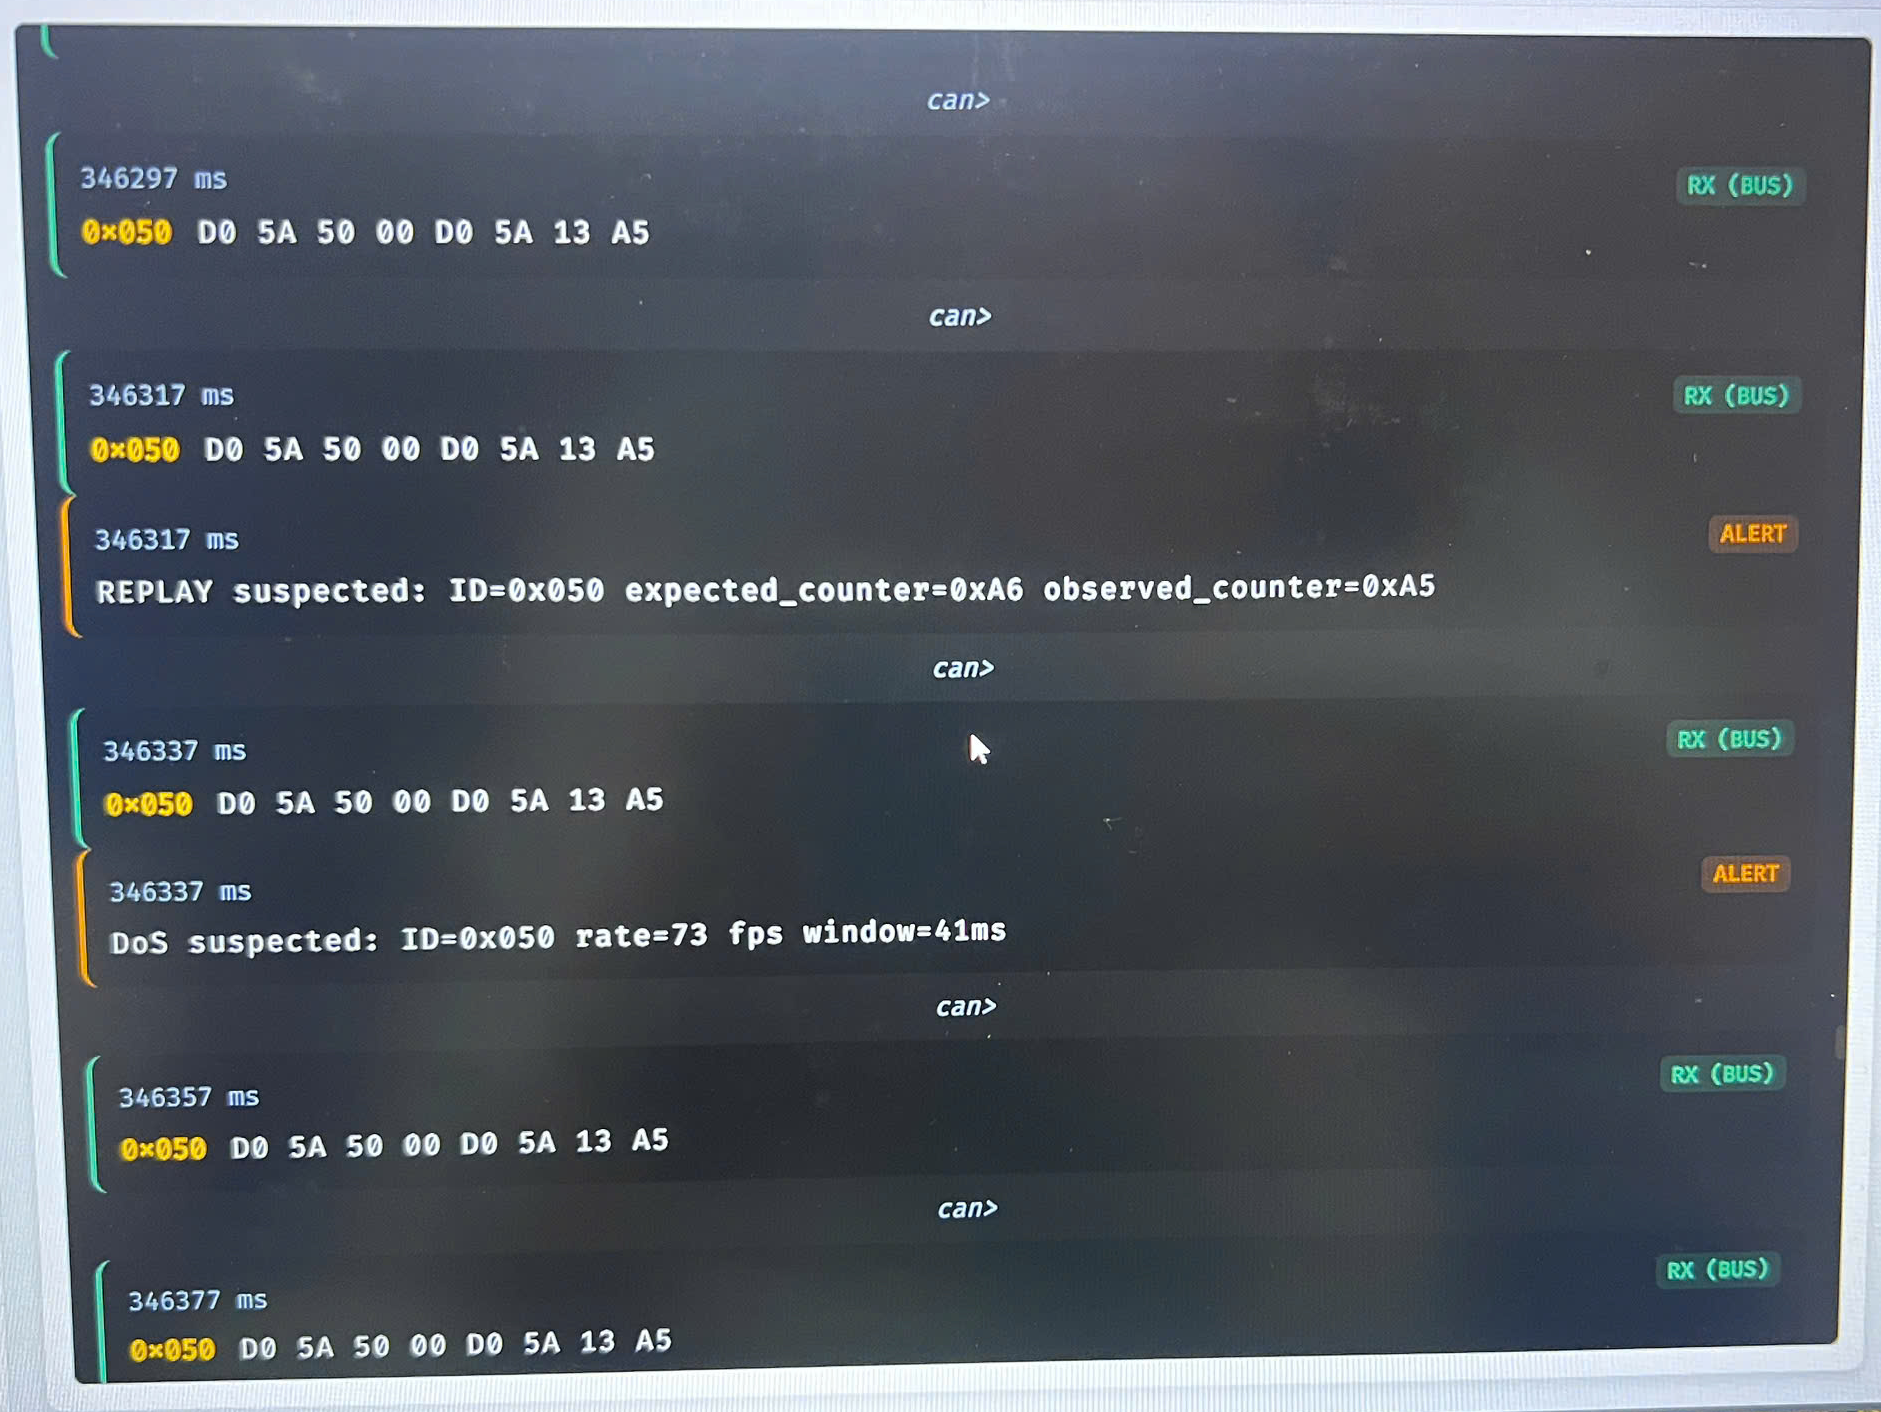
\includegraphics[width=0.98\textwidth]{images/dos_alert.png}
  \caption{Giao diện ghi nhận cảnh báo ở giai đoạn phát hiện tấn công DoS}
  \label{fig:dos-alert}
\end{figure}
}{%
\placeholderfigure{Ảnh giao diện web khi xuất hiện cảnh báo DoS suspected trên nút nhận}{Giao
diện cảnh báo tấn công DoS}
}

Khi DoS diễn ra, giao diện phía nút nhận thường xuất hiện dày đặc các bản tin RX cùng ID,
trong khi phần cảnh báo có thể hiển thị trạng thái \texttt{DoS suspected}. Trên bus, hiện tượng
này tương ứng với việc số khung hợp lệ tăng mạnh trong một cửa sổ thời gian ngắn.

\textbf{Bước cảnh báo:} Ở Hình \ref{fig:dos-alert}, các khung RX với ID \texttt{0x050} xuất hiện
liên tiếp trên giao diện,
đồng thời hệ thống sinh ra nhãn \texttt{ALERT} với dòng \texttt{DoS suspected}. Điều này cho
thấy bộ phát hiện đã nhận ra tốc độ khung tăng bất thường và đánh dấu đây là một phiên có dấu
hiệu ngập lưu lượng. Trong ảnh còn có thêm một dòng \texttt{REPLAY suspected} xuất hiện
trước đó, nhưng trọng tâm của bước này là cảnh báo \texttt{DoS suspected} dùng để kích hoạt
cơ chế phòng thủ ở bước tiếp theo.

\IfFileExists{images/dos_defend.png}{%
\begin{figure}[H]
  \centering
  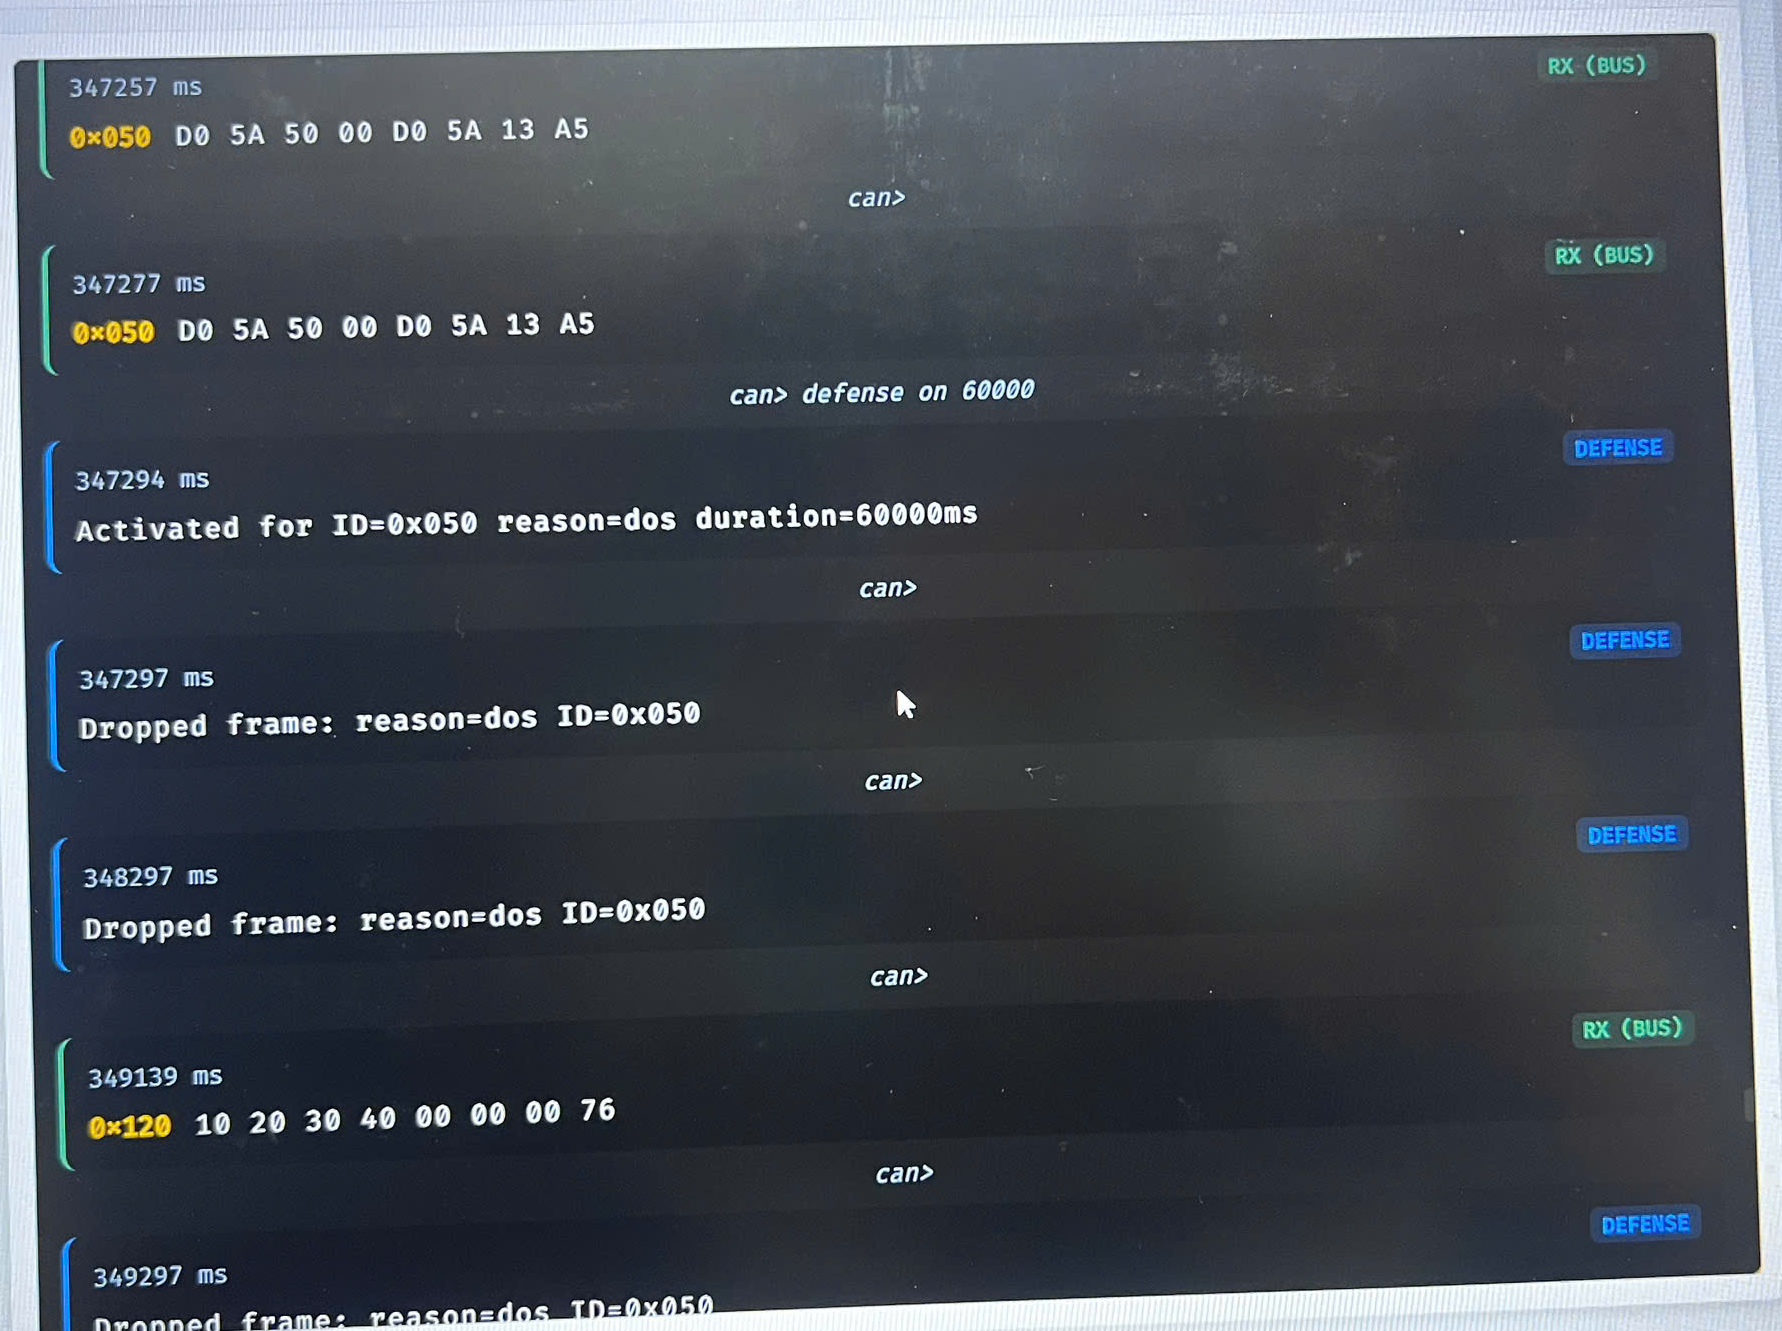
\includegraphics[width=0.98\textwidth]{images/dos_defend.png}
  \caption{Giao diện sau khi bật defense để chặn lưu lượng DoS}
  \label{fig:dos-defend}
\end{figure}
}{%
\placeholderfigure{Ảnh log hiển thị cảnh báo DoS và các khung bị chặn sau khi bật phòng thủ}{Phòng
thủ đối với kịch bản DoS}
}

\textbf{Bước phòng thủ:} Ở Hình \ref{fig:dos-defend}, sau khi người vận hành gửi lệnh
\texttt{defense on 60000}, hệ thống xác nhận kích hoạt phòng thủ bằng thông báo
\texttt{Activated for ID=0x050 reason=dos}. Ngay sau đó, các khung tiếp theo thuộc ID nghi
ngờ không còn được xử lý như dữ liệu hợp lệ mà bị ghi nhận dưới dạng \texttt{Dropped frame}.
Kết quả này cho thấy cơ chế \textit{defend} không làm mất hoàn toàn lưu lượng trên bus vật lý,
nhưng đã chặn được tác động của luồng DoS lên tầng ứng dụng ở nút nhận.

\reportsubsection{2. Tấn công Replay}

Kịch bản Replay yêu cầu nút tấn công đã quan sát được ít nhất một khung hợp lệ trên bus
trước khi phát lại. Sau khi lệnh \texttt{replay start} được kích hoạt, khung vừa thu sẽ được gửi
lặp theo chu kỳ định sẵn, nhằm kiểm tra khả năng phát hiện khung lặp của hệ thống.

\IfFileExists{images/replay_alert.png}{%
\begin{figure}[H]
  \centering
  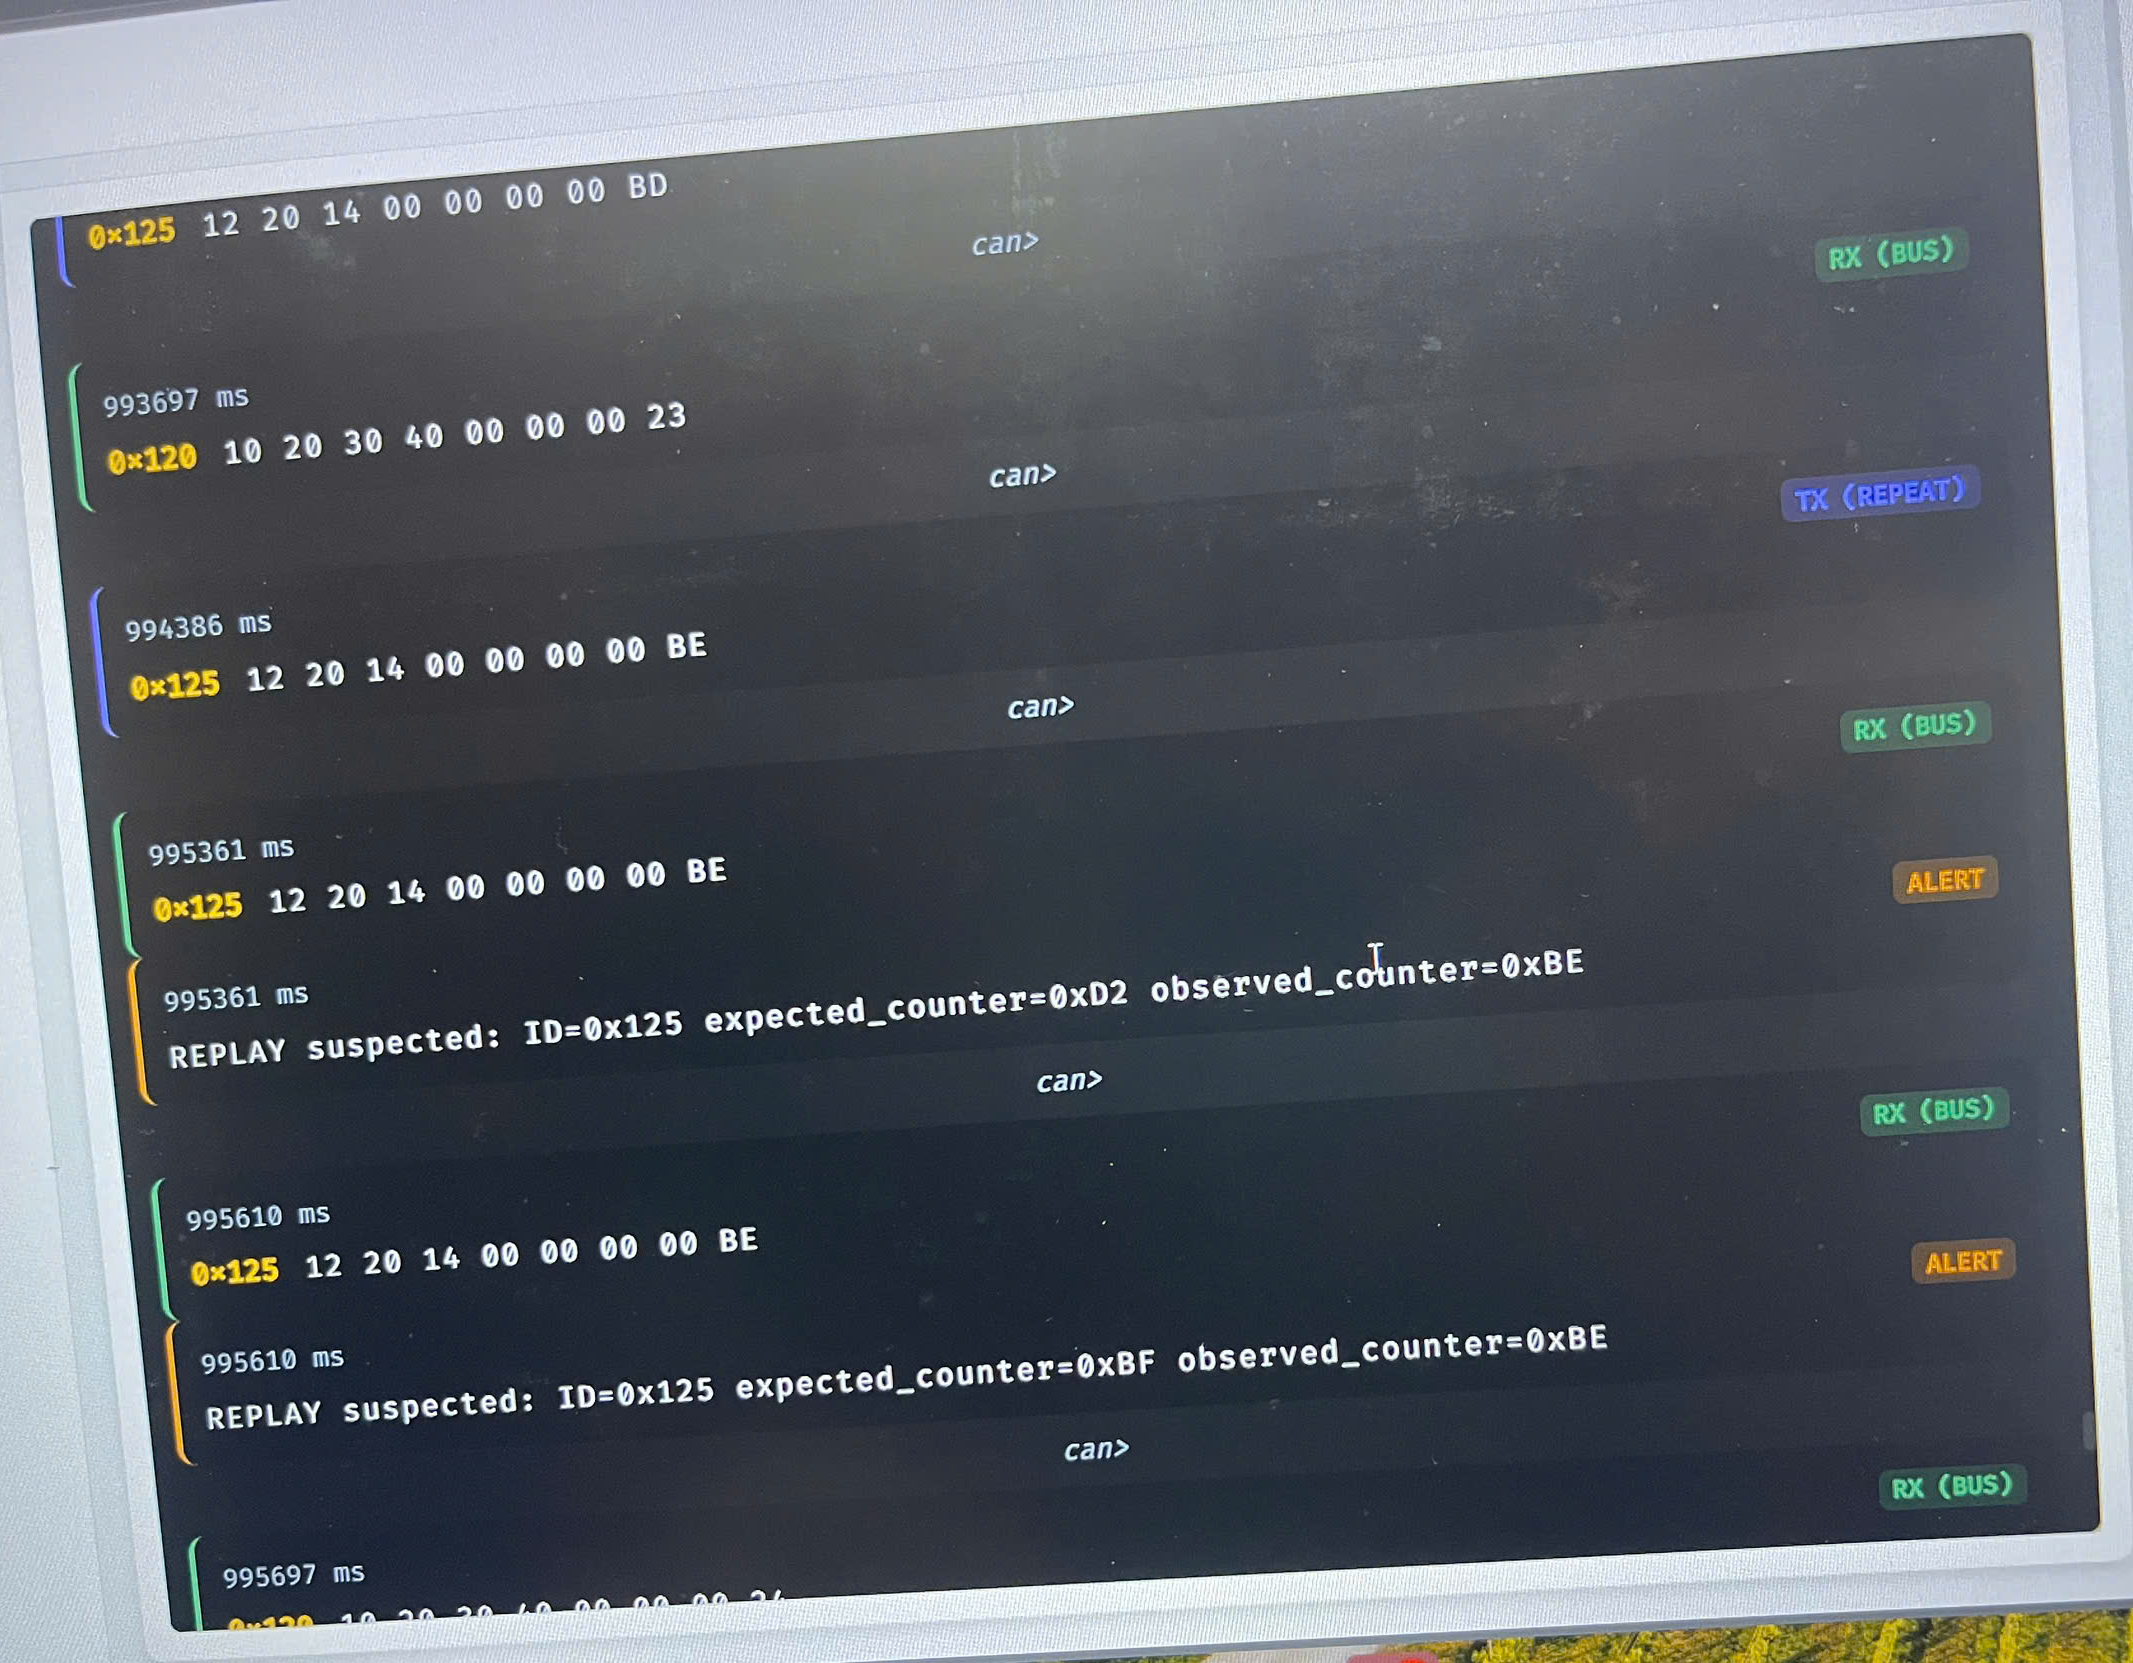
\includegraphics[width=0.9875\textwidth]{images/replay_alert.png}
  \caption{Giao diện ghi nhận cảnh báo ở giai đoạn phát hiện tấn công Replay}
  \label{fig:replay-alert}
\end{figure}
}{%
\placeholderfigure{Ảnh giao diện hoặc terminal khi xuất hiện cảnh báo replay trên nút nhận}{Cảnh
báo tấn công Replay}
}

\IfFileExists{images/replay_defend.png}{%
\begin{figure}[H]
  \centering
  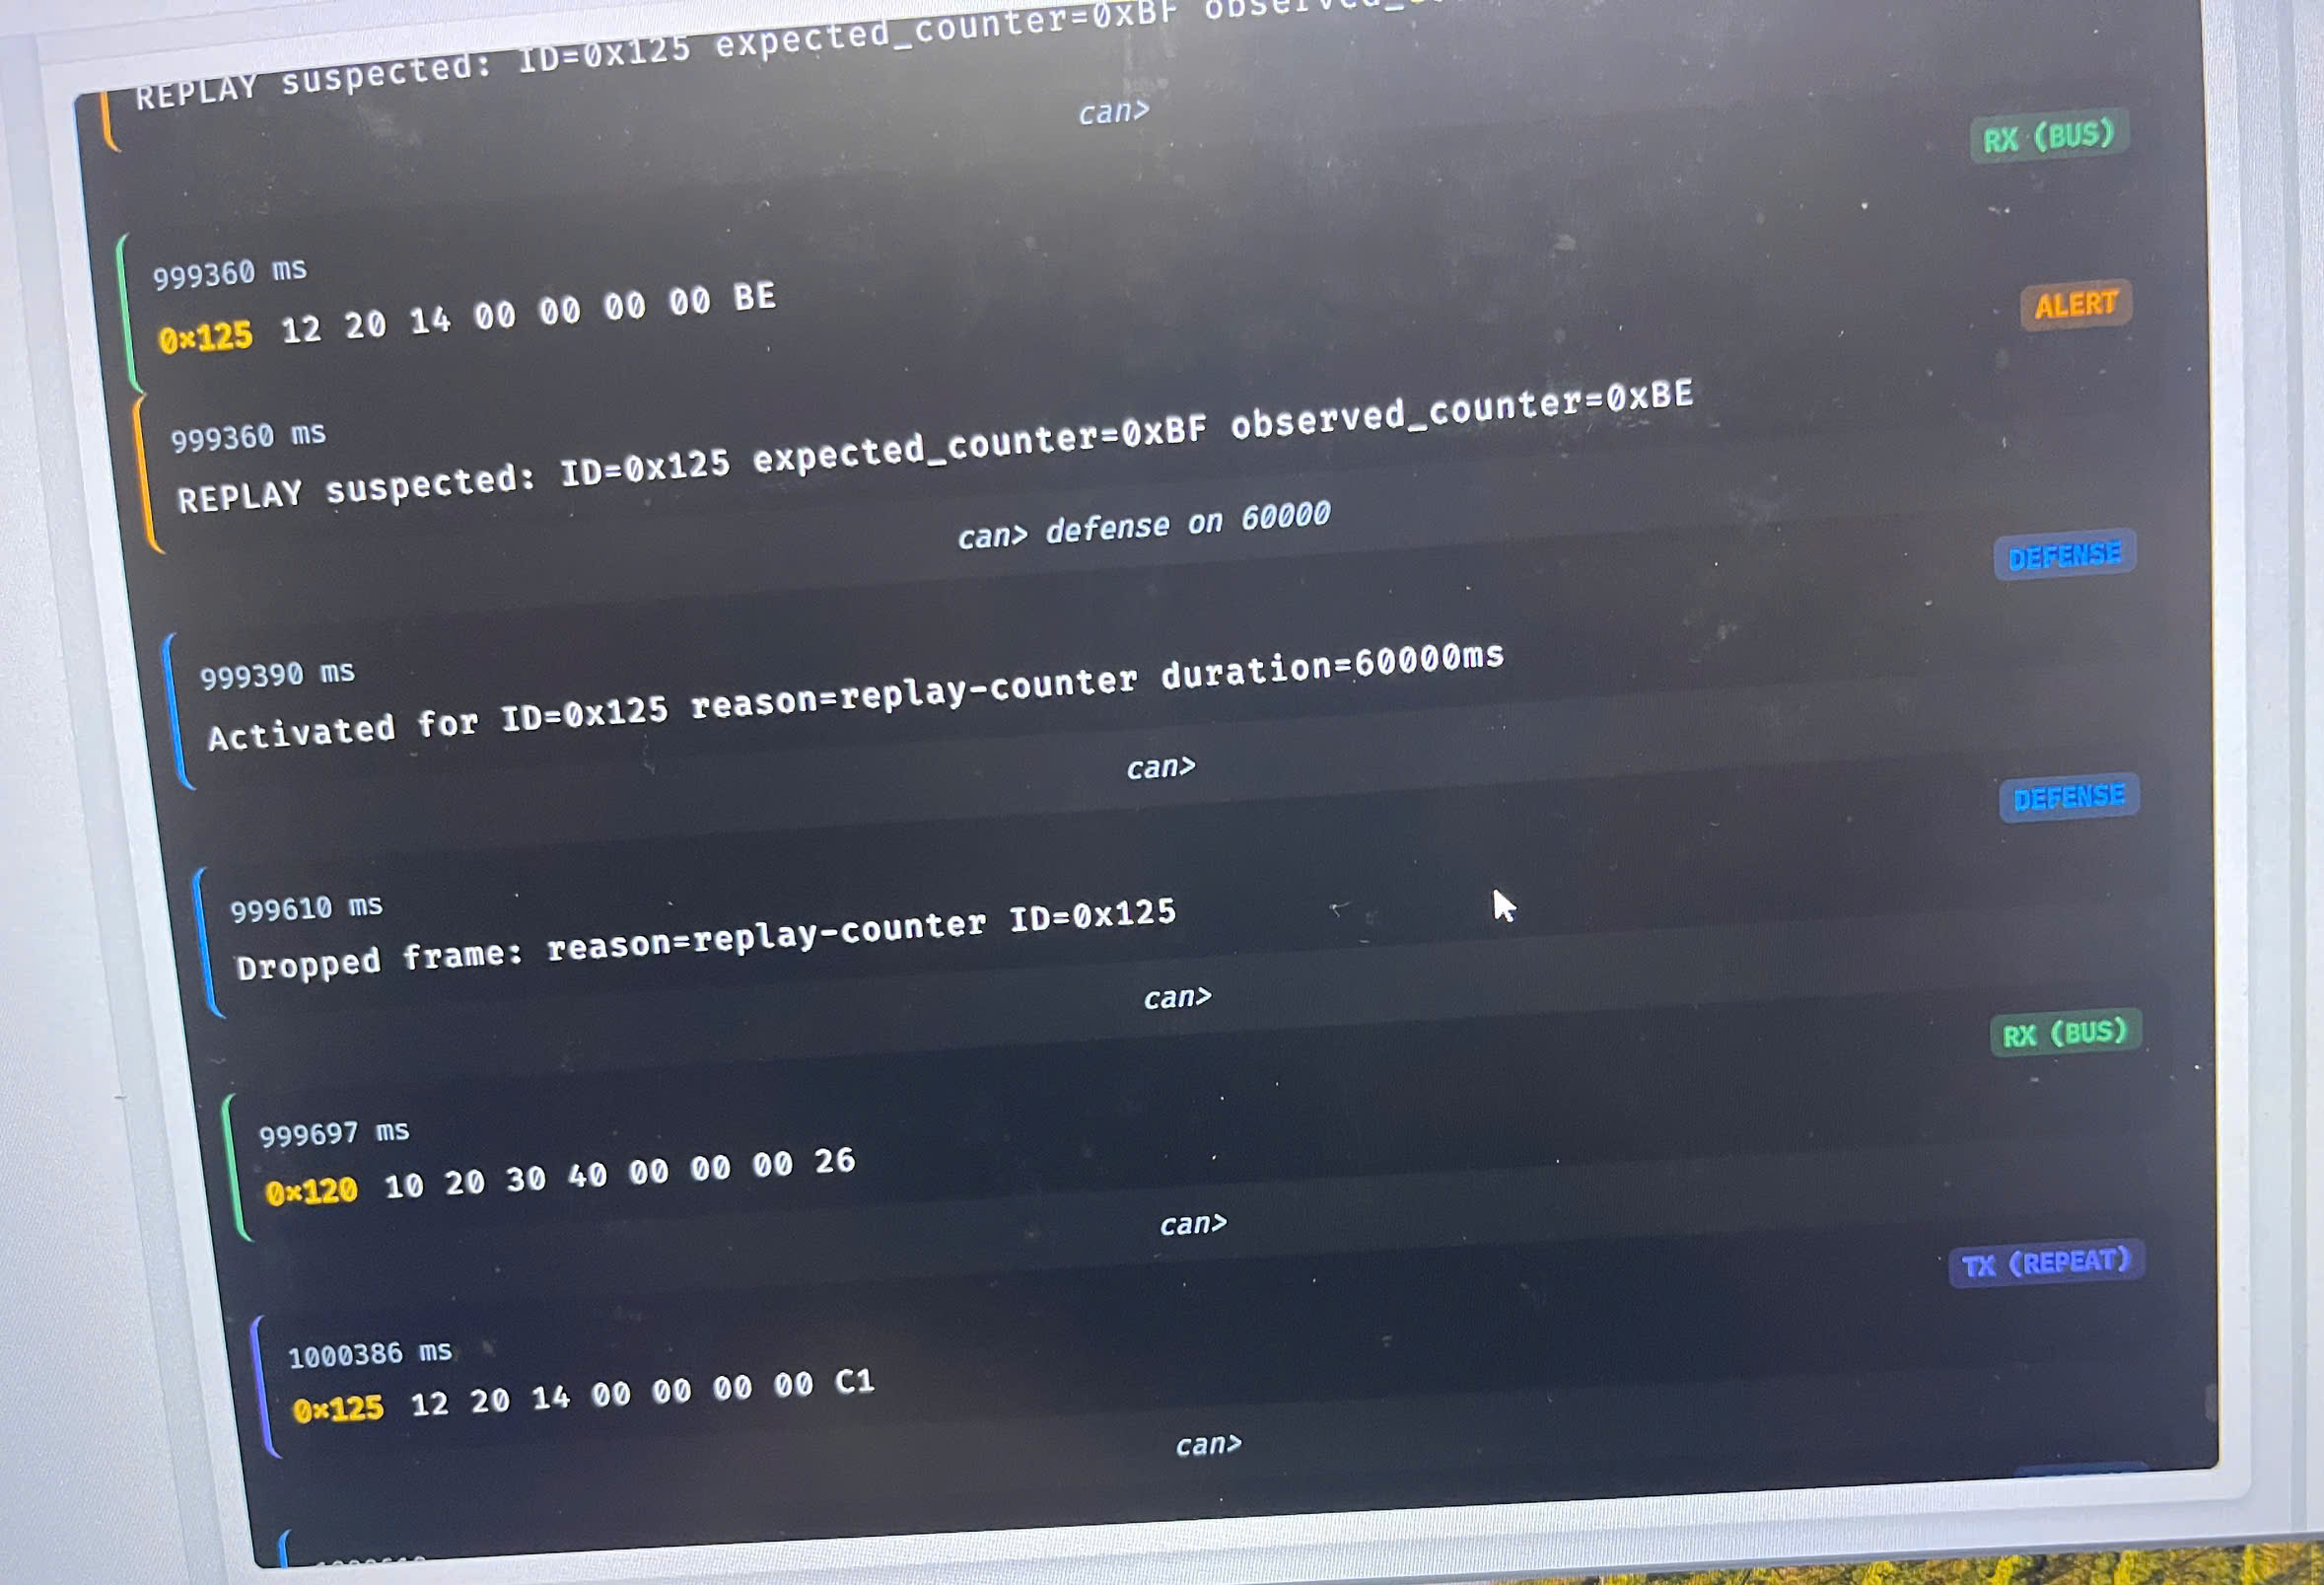
\includegraphics[width=0.75\textwidth]{images/replay_defend.png}
  \caption{Giao diện sau khi bật defense để chặn khung replay}
  \label{fig:replay-defend}
\end{figure}
}{%
\placeholderfigure{Ảnh log hiển thị trạng thái defense và các khung replay bị chặn}{Phòng thủ đối
với kịch bản Replay}
}

{\hbadness=10000
\textbf{Bước cảnh báo:} Ở Hình \ref{fig:replay-alert}, hệ thống tại nút nhận liên tục quan sát
thấy các khung mang ID \texttt{0x125} có giá trị bộ đếm cũ bị lặp lại. Hệ thống tiến hành so sánh
bộ đếm quan sát được với bộ đếm kỳ vọng và sinh ra cảnh báo \texttt{REPLAY suspected}, ví dụ
\texttt{expected\_counter=0xD2} \texttt{observed\_counter=0xBE}. Điều này minh chứng rằng cùng một
khung đã bị phát lại thay vì tiếp tục tăng tuần tự như trong phiên truyền hợp lệ.\par}

\textbf{Bước phòng thủ:} Ở Hình \ref{fig:replay-defend}, sau khi người vận hành gửi lệnh
\texttt{defense on 60000}, hệ thống xác nhận kích hoạt phòng thủ bằng thông báo
\texttt{Activated for ID=0x125 reason=replay-counter duration=60000ms}. Ngay sau đó, các
khung replay tiếp theo không còn được xử lý như dữ liệu hợp lệ mà bị ghi nhận dưới dạng
\texttt{Dropped frame: reason=replay-counter ID=0x125}. Cơ chế này giúp chặn luồng phát lại ở
tầng ứng dụng trong khi việc giám sát bus vẫn tiếp tục diễn ra.

\reportsubsection{3. Tấn công Fuzzing}

Trong kịch bản Fuzzing, nút tấn công liên tục thay đổi ID và dữ liệu tải để tạo ra chuỗi bản tin
bất thường, khó dự đoán. Mục tiêu của phần này là đánh giá khả năng phát hiện sự thay đổi
nhanh về mẫu lưu lượng, đặc biệt khi số lượng ID khác nhau tăng lên trong thời gian ngắn.

\IfFileExists{images/fuzzing_alert.png}{%
\begin{figure}[H]
  \centering
  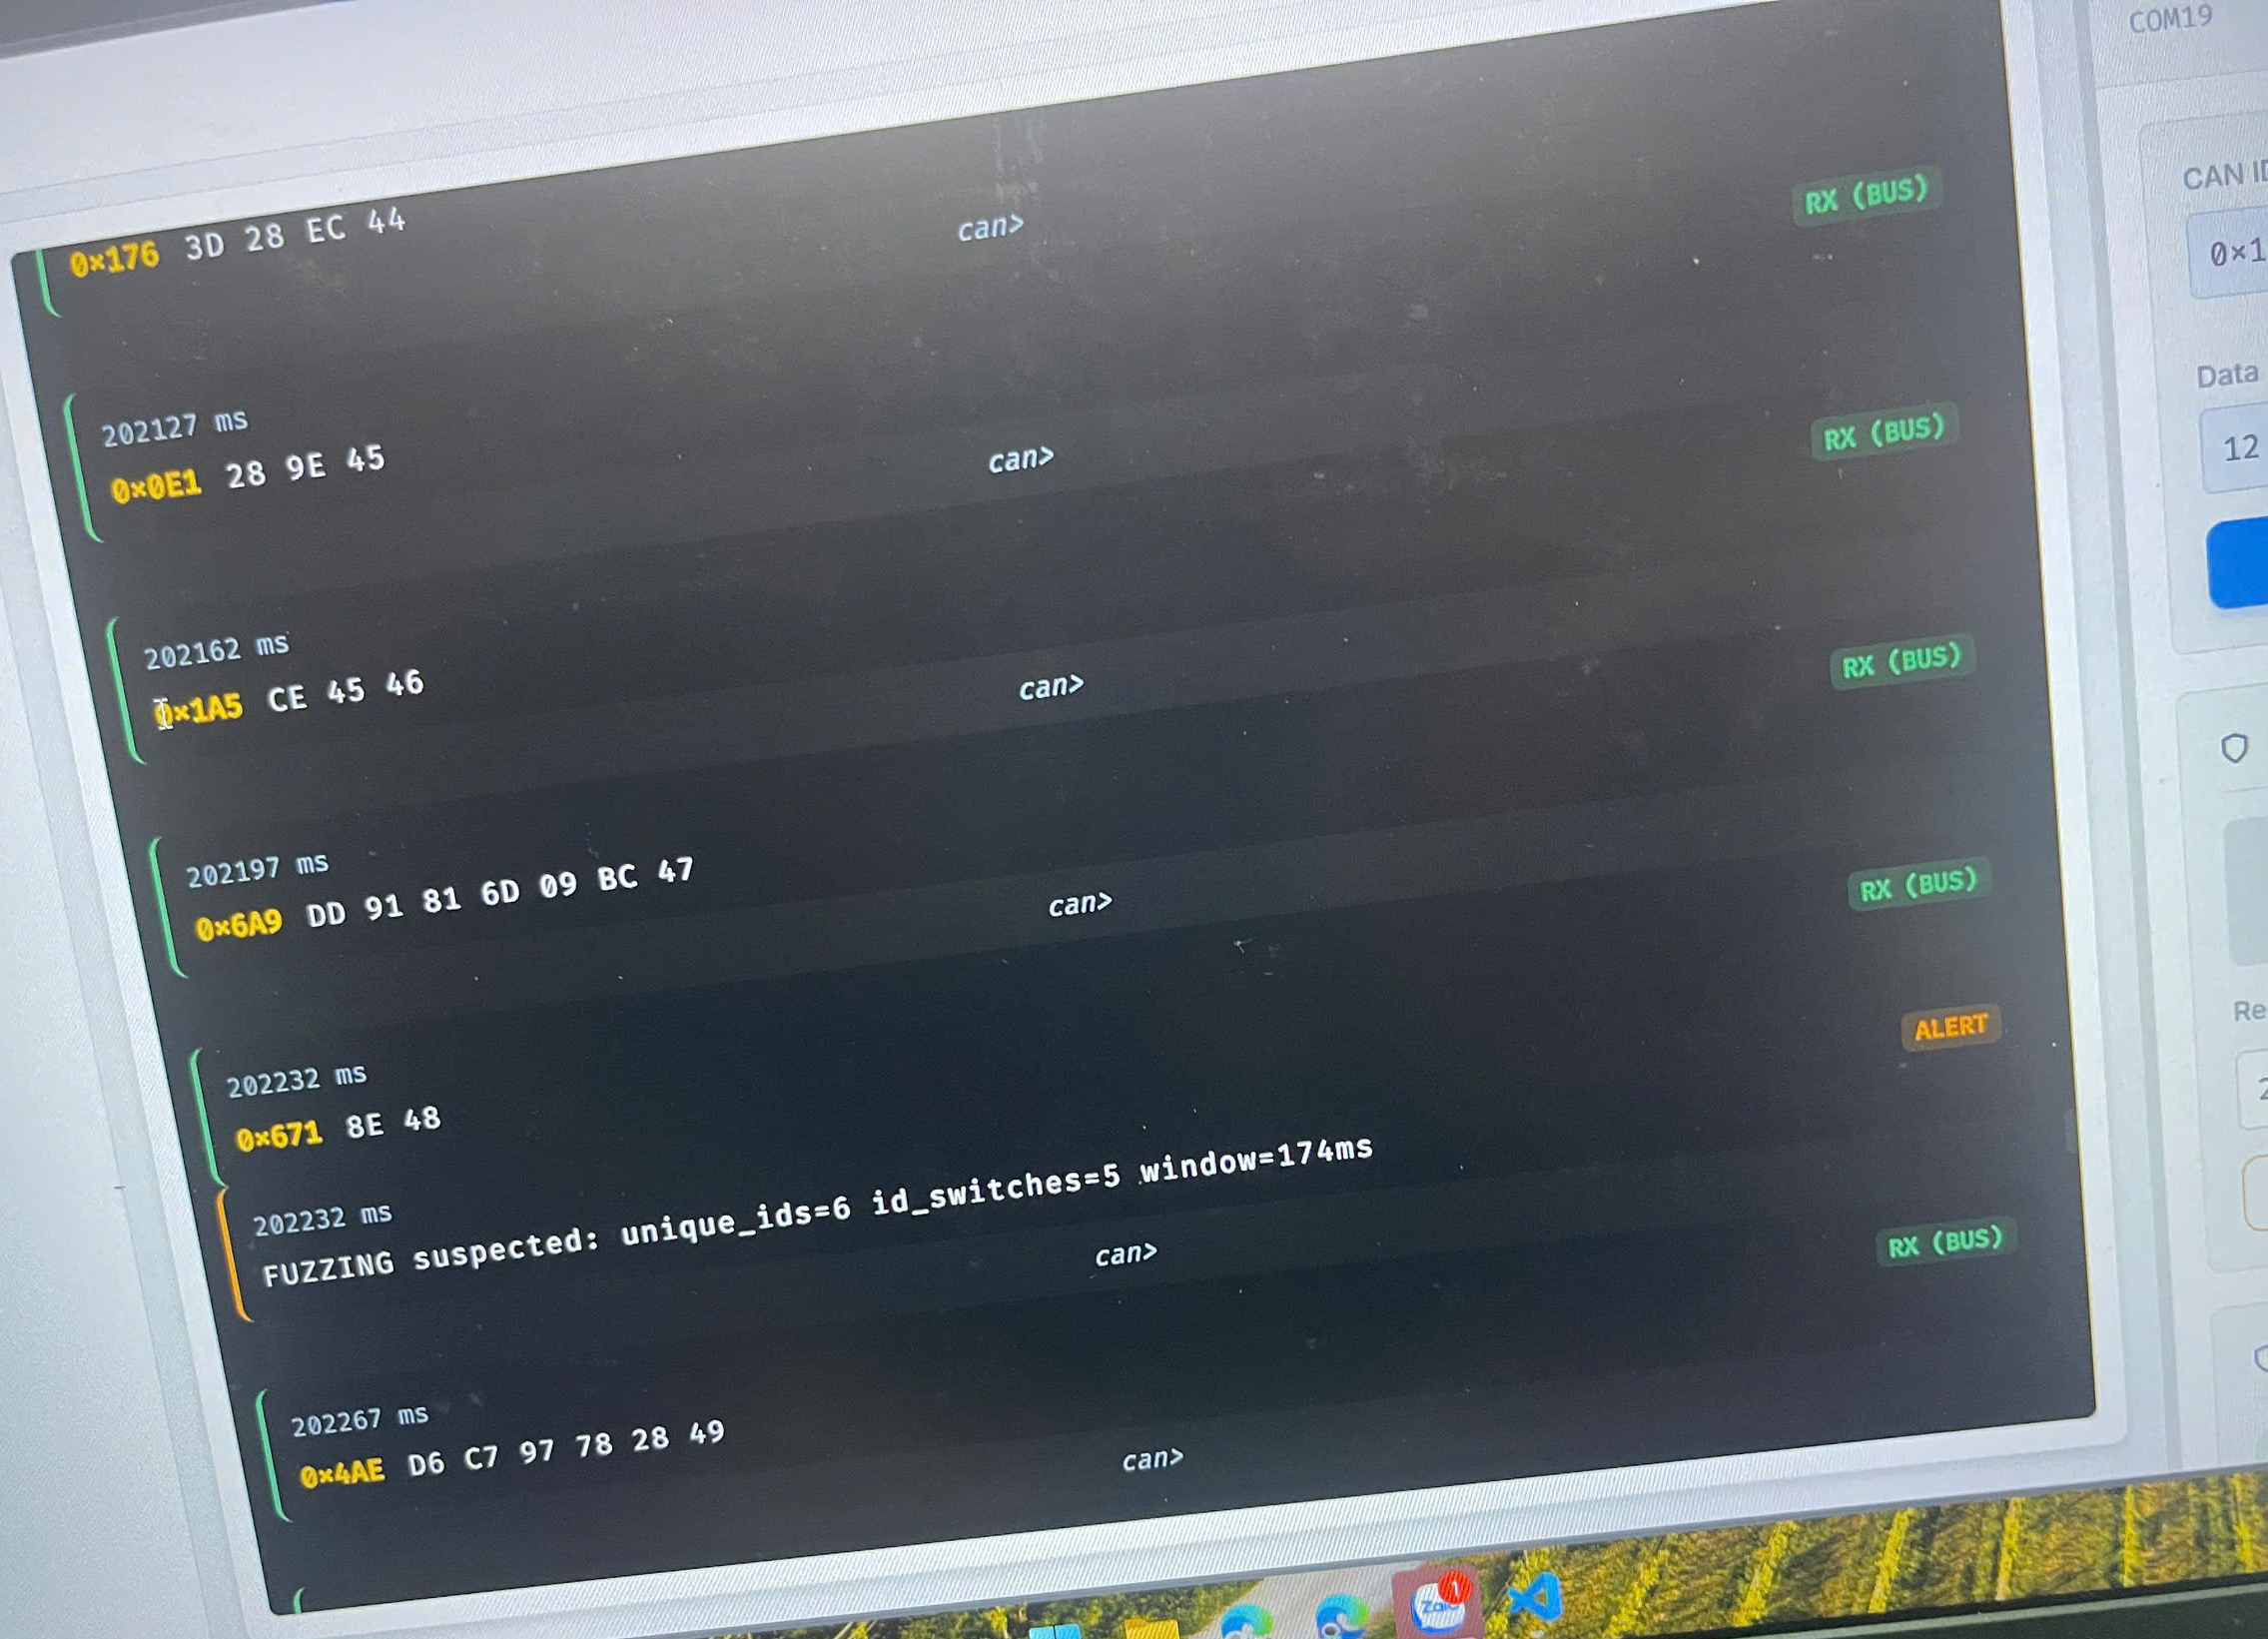
\includegraphics[width=0.98\textwidth]{images/fuzzing_alert.png}
  \caption{Giao diện ghi nhận cảnh báo ở giai đoạn phát hiện tấn công Fuzzing}
  \label{fig:fuzzing-alert}
\end{figure}
}{%
\placeholderfigure{Ảnh giao diện web khi xuất hiện cảnh báo fuzzing trên nút nhận}{Cảnh báo tấn
công Fuzzing}
}

Khi quan sát ở nút nhận, các bản tin xuất hiện với ID thay đổi nhanh và nội dung dữ liệu không
ổn định như trong chế độ truyền bình thường. Trong log, hệ thống có thể sinh cảnh báo
\texttt{FUZZING suspected} khi số lượng ID khác nhau và tần suất chuyển đổi ID vượt mức
cho phép.

\IfFileExists{images/fuzzing_defend.png}{%
\begin{figure}[H]
  \centering
  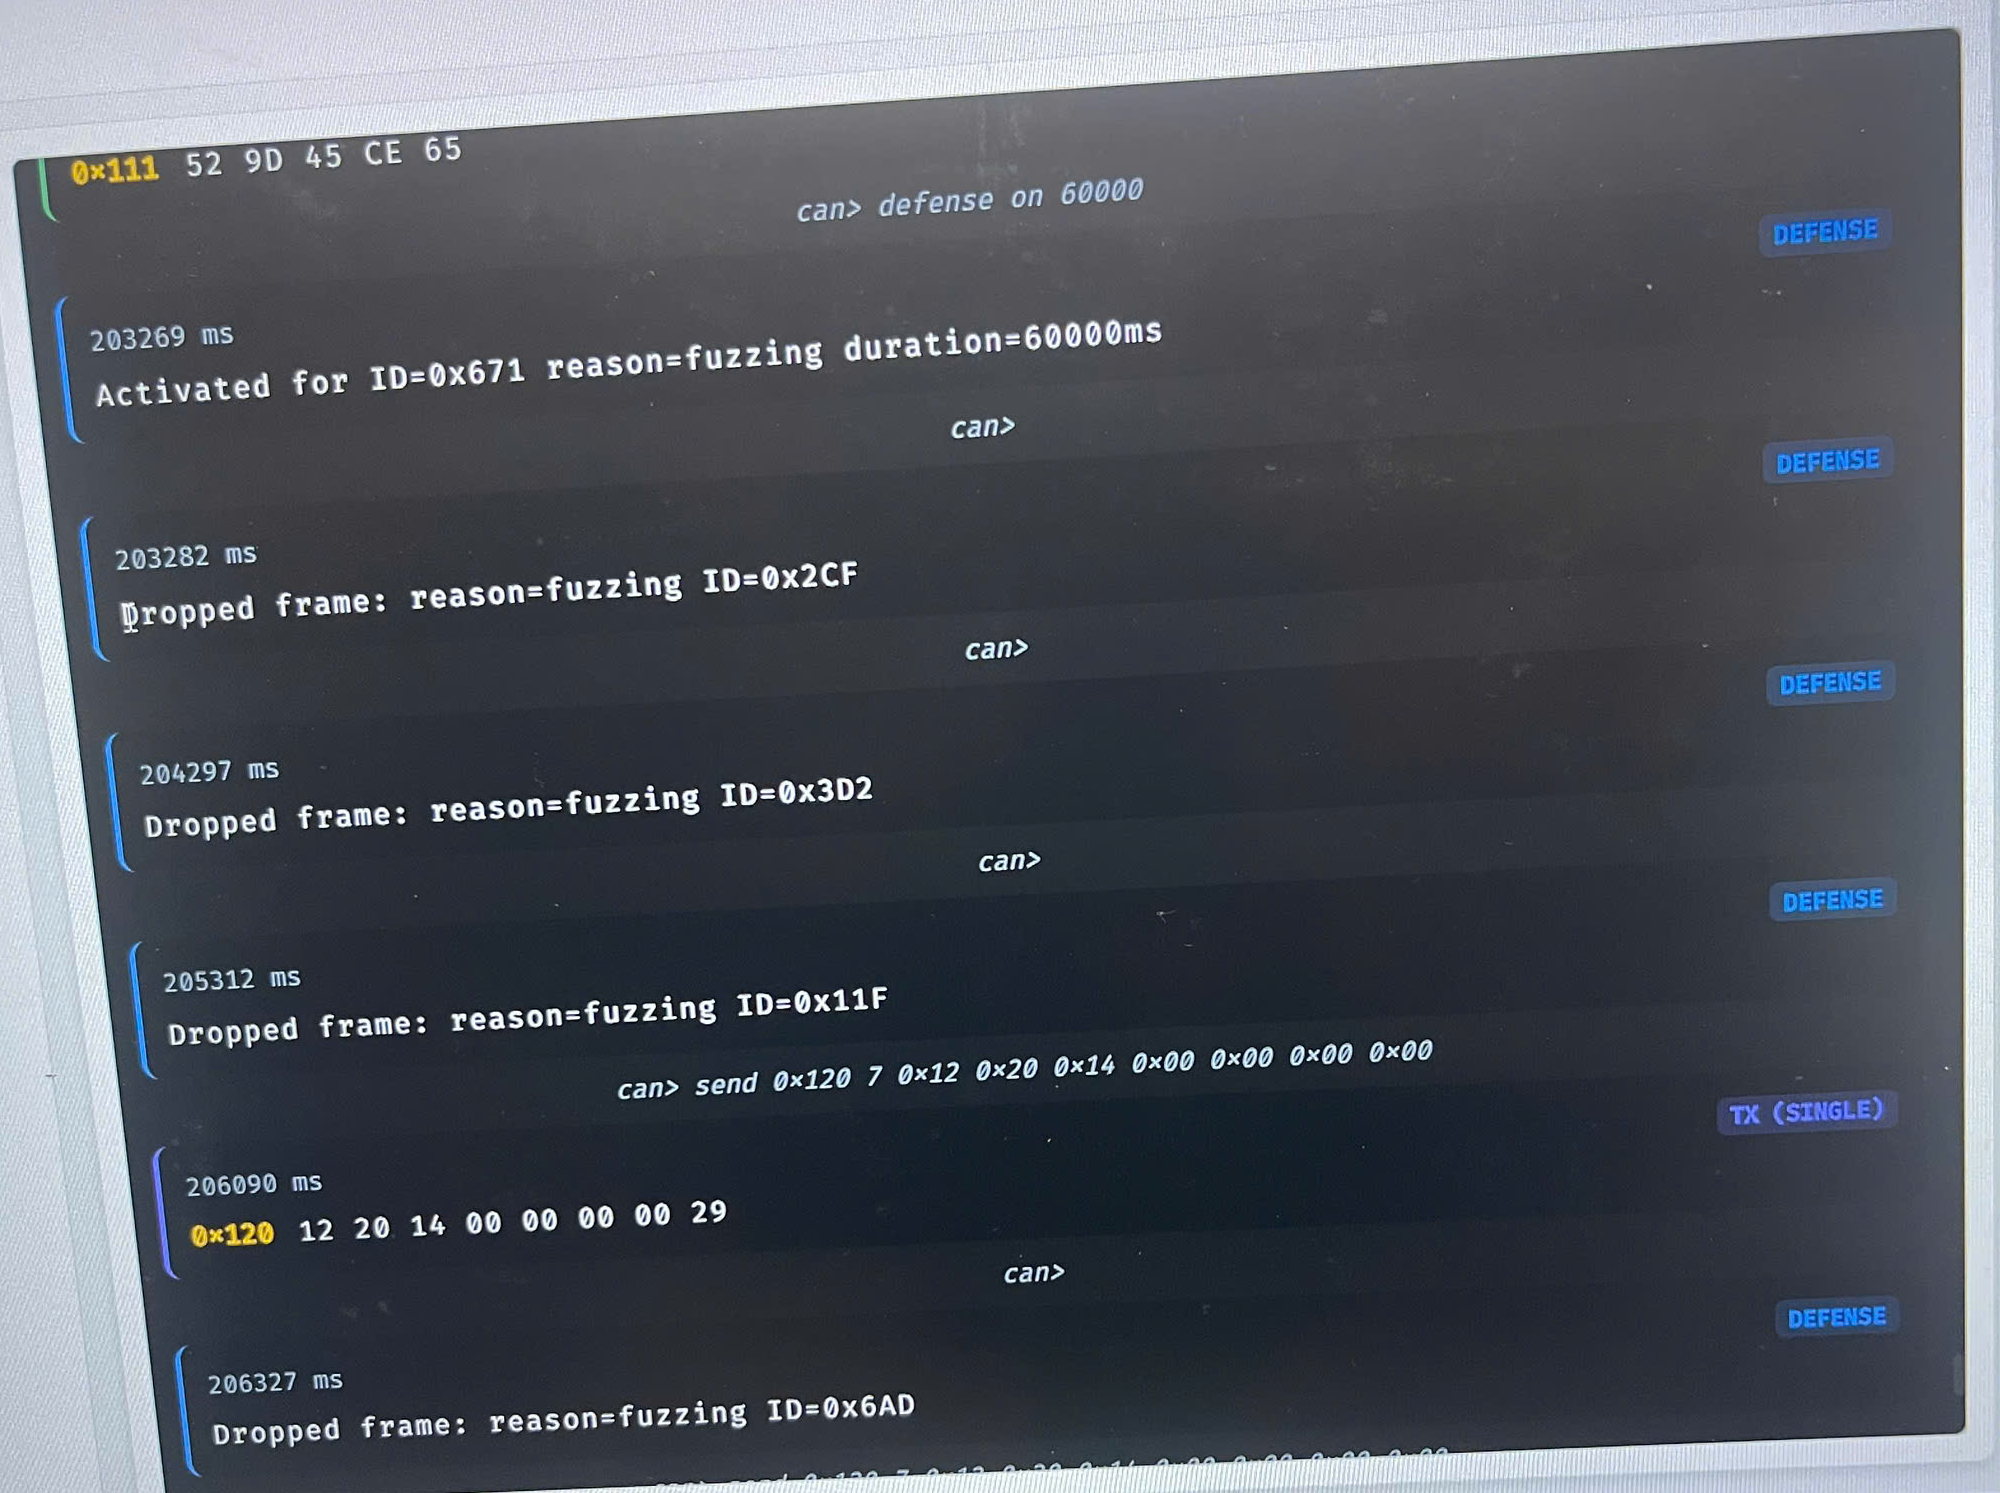
\includegraphics[width=0.98\textwidth]{images/fuzzing_defend.png}
  \caption{Giao diện sau khi bật defense để chặn lưu lượng Fuzzing}
  \label{fig:fuzzing-defend}
\end{figure}
}{%
\placeholderfigure{Ảnh log hiển thị trạng thái defense và các khung fuzzing bị chặn}{Phòng thủ đối
với kịch bản Fuzzing}
}

\textbf{Bước cảnh báo:} Ở Hình \ref{fig:fuzzing-alert}, nút nhận quan sát liên tiếp nhiều khung với
CAN ID thay đổi nhanh như \texttt{0x176}, \texttt{0x0E1}, \texttt{0x1A5}, \texttt{0x6A9},
\texttt{0x671}. Khi số lượng ID khác nhau và số lần chuyển đổi ID vượt ngưỡng, hệ thống sinh
cảnh báo \texttt{FUZZING suspected: unique\_ids=6 id\_switches=5 window=174ms}. Điều này
cho thấy lưu lượng đang bị tiêm nhiễu với mẫu phát không còn ổn định như giao tiếp bình
thường.

{\hbadness=10000
\textbf{Bước phòng thủ:} Ở Hình \ref{fig:fuzzing-defend}, ngay sau khi người vận hành tiến hành
gửi lệnh \texttt{defense on 60000}, hệ thống lập tức xác nhận kích hoạt thông qua thông báo
\texttt{Activated for ID=0x671} \texttt{reason=fuzzing} \texttt{duration=60000ms}. Sau đó, nhiều khung
lạ tiếp tục xuất hiện trên bus nhưng đã bị chặn ngay ở tầng ứng dụng với các dòng ghi log
\texttt{Dropped frame:} \texttt{reason=fuzzing} \texttt{ID=...}. Kết quả này chứng minh cơ chế phòng thủ
đã cô lập thành công luồng fuzzing mà vẫn cho phép các bản tin hợp lệ tiếp tục được quan sát.\par}

\reportsubsection{4. Tấn công Spoofing}

Trong kịch bản Spoofing, nút tấn công phát khung với cùng CAN ID của một thông điệp hợp lệ
nhưng thay đổi phần dữ liệu tải để giả mạo nội dung. Trước khi bắt đầu phần này, nên cho nút
hợp lệ gửi vài lần cùng một ID để hệ thống phía nhận có cơ sở xây dựng mẫu dữ liệu nền.

\IfFileExists{images/spoof_alert.png}{%
\begin{figure}[H]
  \centering
  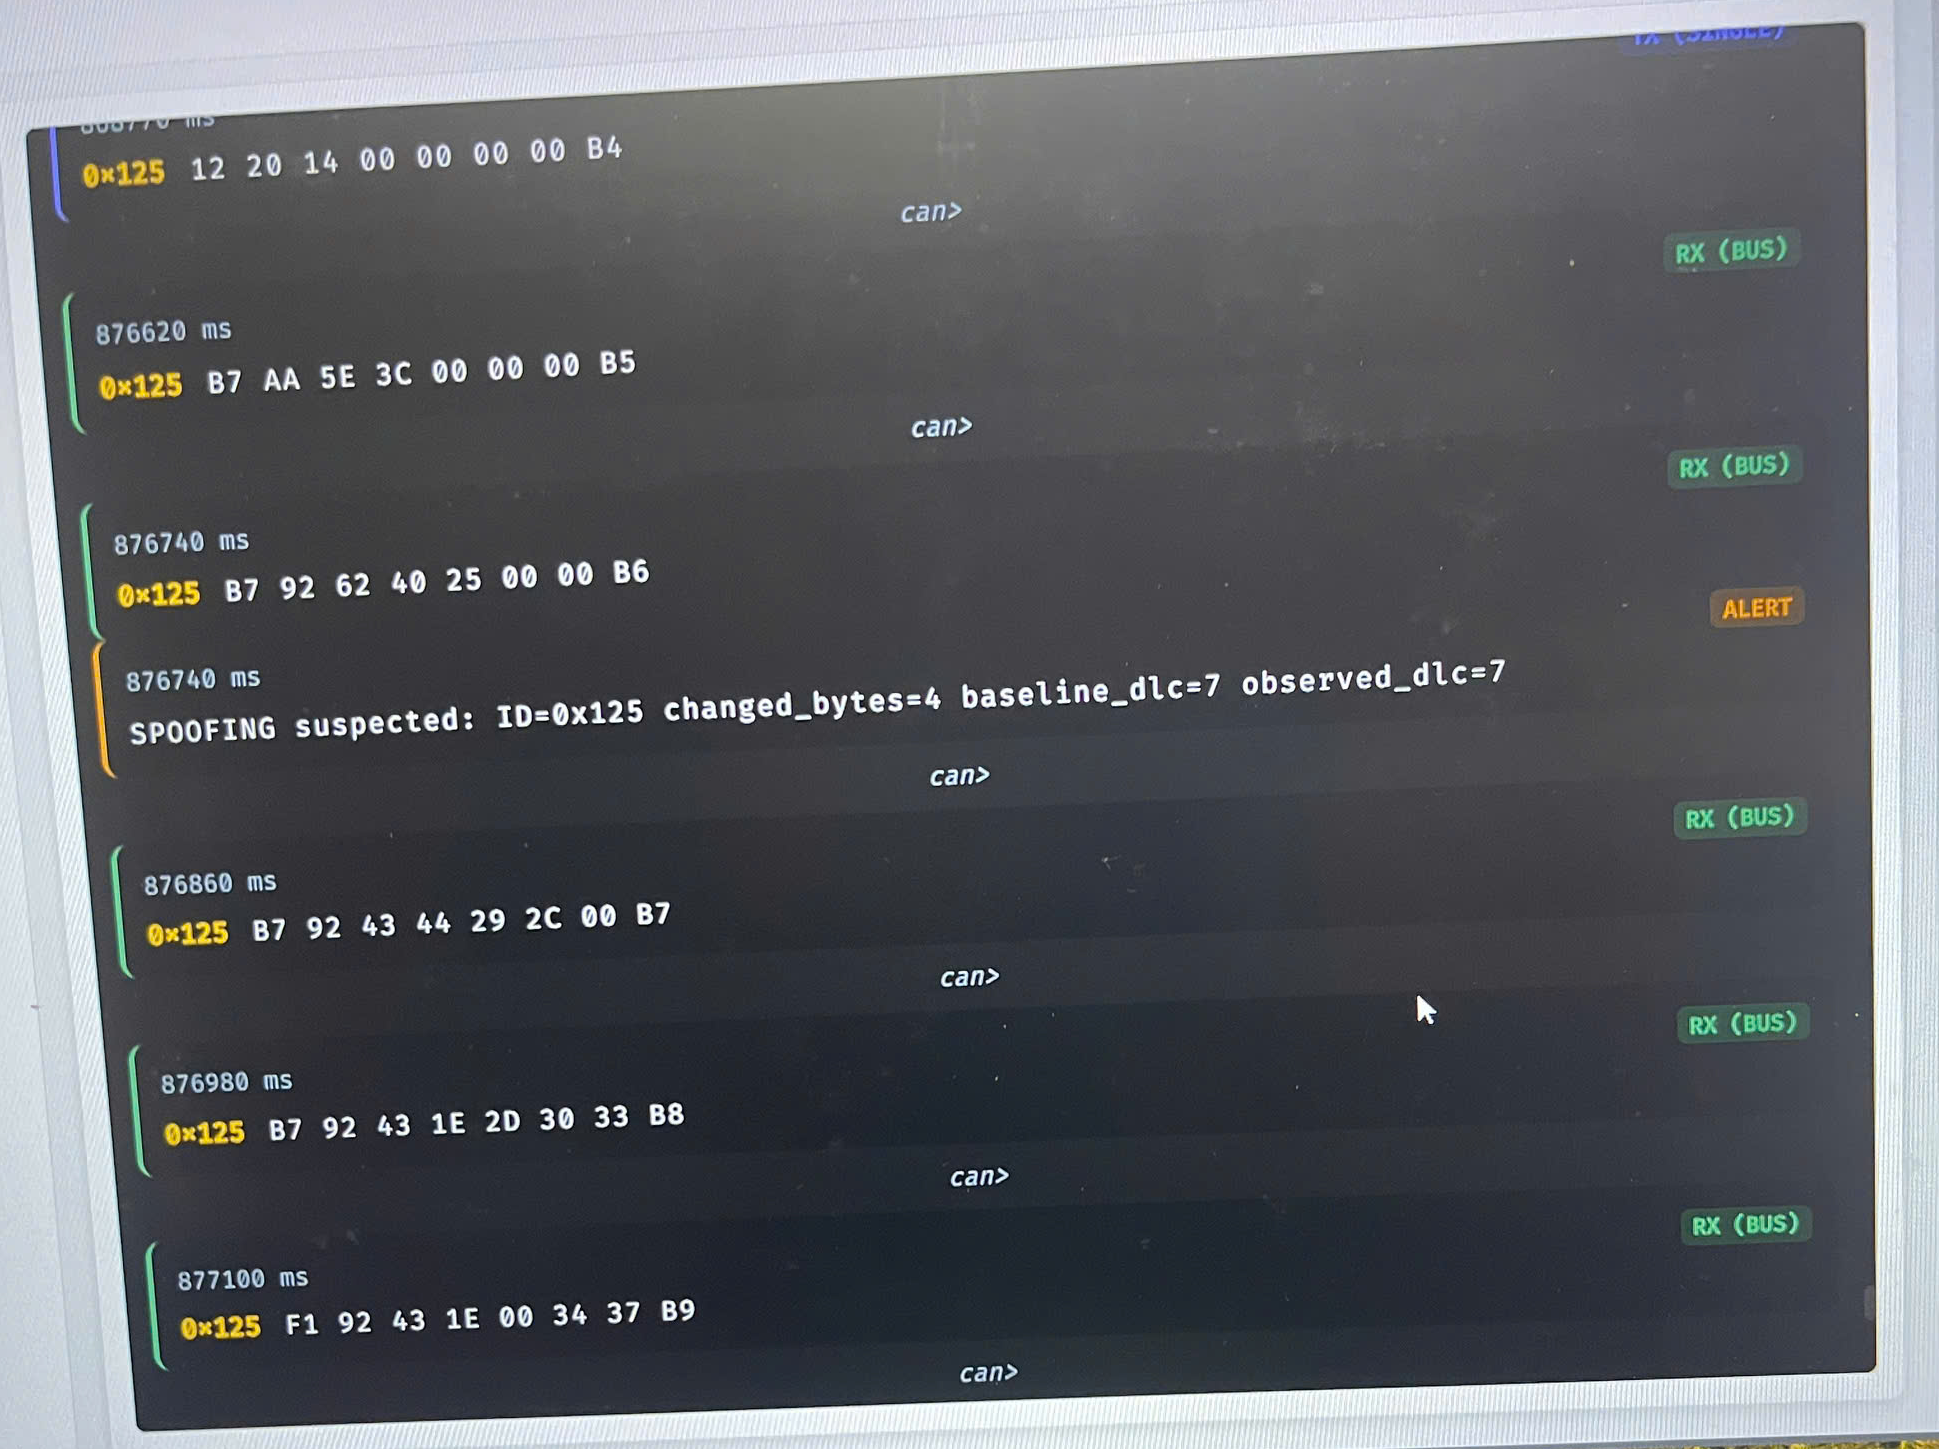
\includegraphics[width=0.98\textwidth]{images/spoof_alert.png}
  \caption{Giao diện ghi nhận cảnh báo ở giai đoạn phát hiện tấn công Spoofing}
  \label{fig:spoof-alert}
\end{figure}
}{%
\placeholderfigure{Ảnh giao diện khi xuất hiện cảnh báo spoofing trên nút nhận}{Cảnh báo tấn
công Spoofing}
}

Khi spoofing diễn ra, phía nhận vẫn thấy cùng một CAN ID quen thuộc nhưng phần dữ liệu thay
đổi bất thường so với mẫu hợp lệ trước đó. Đây là cơ sở để hệ thống sinh cảnh báo
\texttt{SPOOFING suspected} và phân biệt khung giả mạo với khung hợp lệ có cùng ID.

\IfFileExists{images/spoof_defend.png}{%
\begin{figure}[H]
  \centering
  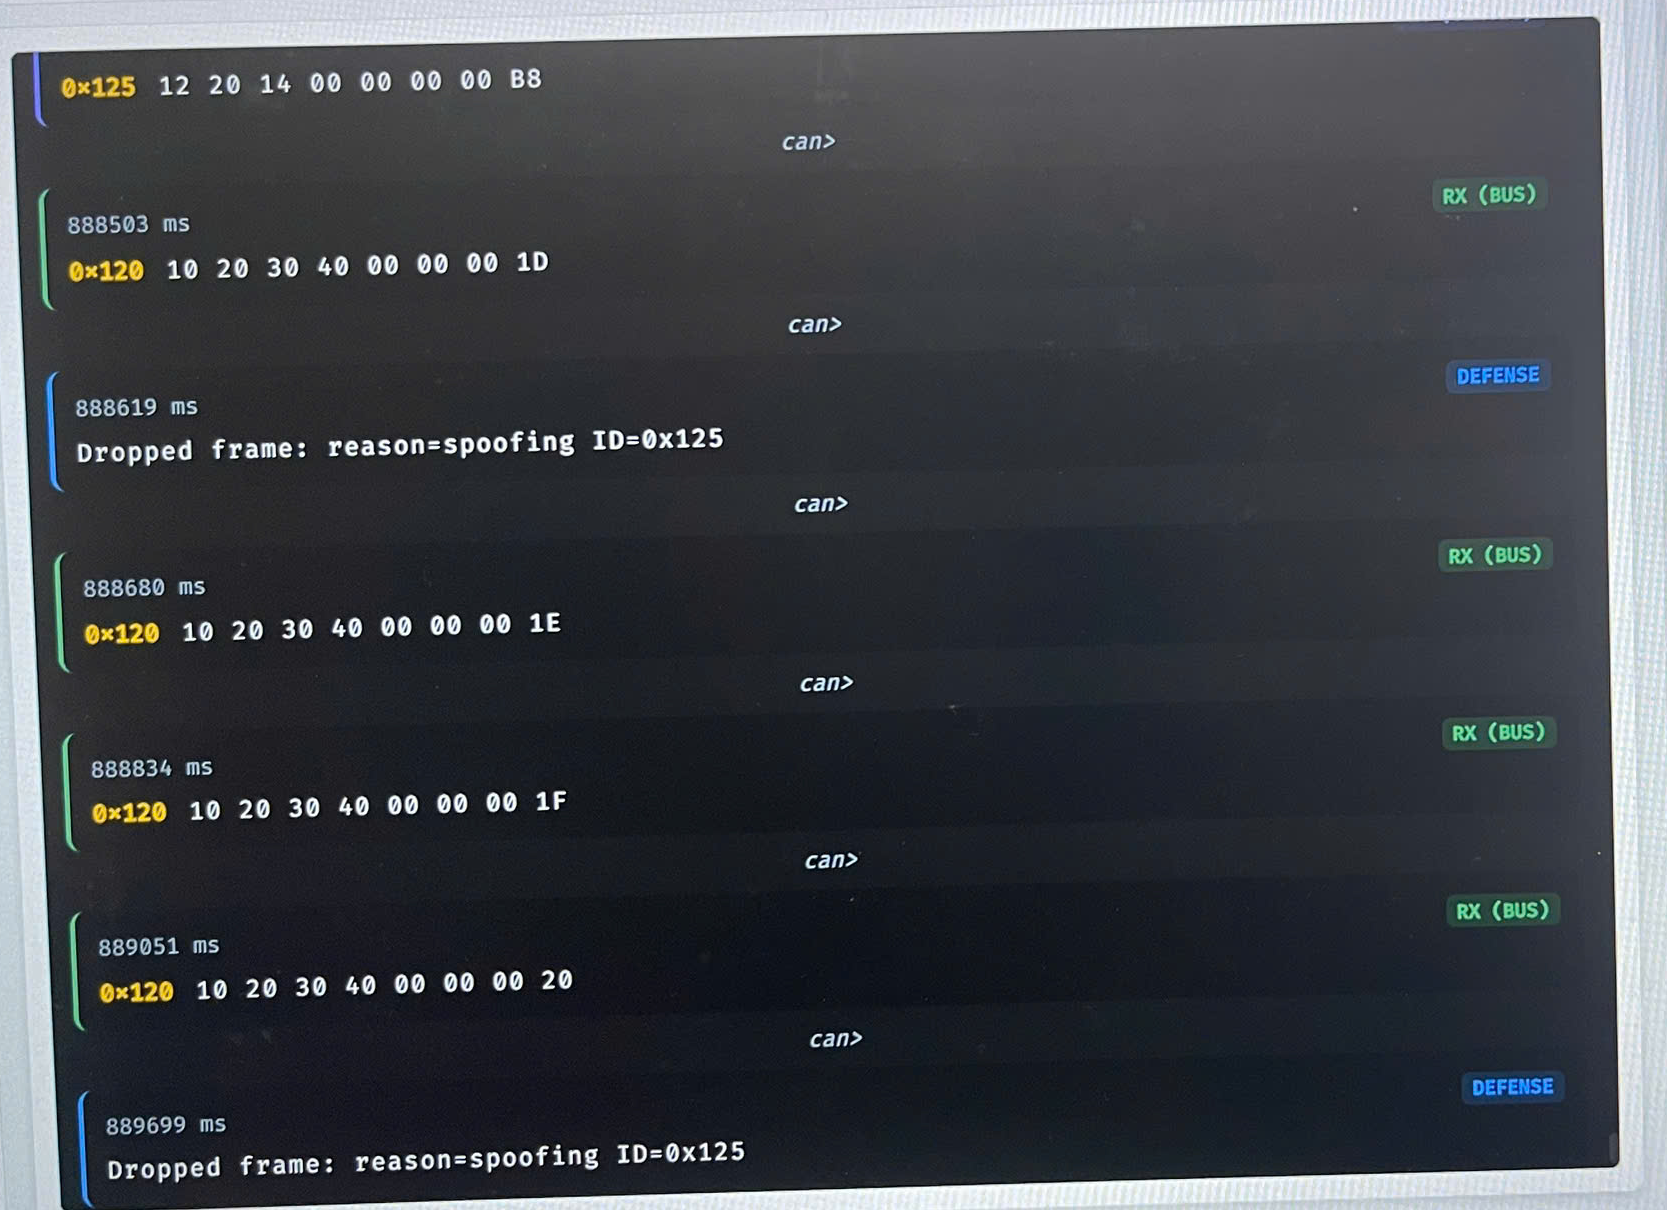
\includegraphics[width=0.98\textwidth]{images/spoof_defend.png}
  \caption{Giao diện sau khi bật defense để chặn khung spoofing}
  \label{fig:spoof-defend}
\end{figure}
}{%
\placeholderfigure{Ảnh log hiển thị trạng thái defense và các khung spoofing bị chặn}{Phòng thủ
đối với kịch bản Spoofing}
}

\textbf{Bước cảnh báo:} Ở Hình \ref{fig:spoof-alert}, nút nhận vẫn quan sát cùng CAN ID
\texttt{0x125} nhưng nội dung payload đã thay đổi rõ rệt so với mẫu hợp lệ trước đó. Từ sự sai
khác này, hệ thống sinh cảnh báo \texttt{SPOOFING suspected:} \texttt{ID=0x125} \texttt{changed\_bytes=4}
\texttt{baseline\_dlc=7} \texttt{observed\_dlc=7}. Đây là dấu hiệu cho thấy một khung giả mạo đang cố chèn
vào luồng giao tiếp bình thường.

\textbf{Bước phòng thủ:} Ở Hình \ref{fig:spoof-defend}, sau khi defense đã được bật, các khung
giả mạo cùng ID \texttt{0x125} không còn được xử lý như dữ liệu hợp lệ mà bị ghi nhận bằng
các dòng \texttt{Dropped frame: reason=spoofing ID=0x125}. Trong khi đó, các khung hợp lệ
khác như \texttt{0x120} vẫn tiếp tục xuất hiện trên giao diện. Điều này cho thấy cơ chế defense
đã chặn được luồng giả mạo theo đúng CAN ID nghi ngờ mà không làm gián đoạn hoàn toàn
quá trình giám sát bus.

Toàn bộ video minh họa cho các bước tấn công và phòng thủ của bốn kịch bản.

\begin{itemize}[leftmargin=*]
  \item \href{https://drive.google.com/drive/folders/1Ofl2Voi7a0QwBnF00v7ZM63E-JsUBCxc?usp=sharing}{\textcolor{blue}{Video tấn công và phòng thủ cho các kịch bản DoS, Replay, Fuzzing, Spoofing}}
\end{itemize}

